\section{Deployment}
This section describes deployment architectures that are possible with Spring XD.
Note that this is not an exhaustive list of all deployment types. See
section~\ref{sec:Use Cases} for descriptions of real world deployments.

\subsection{Lambda Architecture}

The Lambda Architecture, introduced by Nathan Marz \cite{lambda-architecture-paper}
and shown in figure~\ref{fig:lambda}
is a generic, scalable and fault tolerant data  processing architecture. It 
attempts to provide a comprehensive solution to the problem of processing an 
extremely large set of data.

The Lambda Architecture has the following components:

\begin{itemize*}
\item A \emph{master dataset} consisting of all data known to the system,
ideally in its rawest form;
\item A \emph{serving} or \emph{view layer} that provides the latest,
most up-to-date view of the processed data, available for low-latency,
ad-hoc querying;
\item A \emph{batch layer} that performs computationally intense 
calculations and prepares the \emph{batch views} displayed by the 
\emph{serving layer};
\item A \emph{speed layer} that performs calculations on recent data only, 
its output combined with the \emph{batch views} by the \emph{serving layer}.
\end{itemize*}

The guiding principle of the Lambda architecture is to combine the
high throughput of batch operations with the low latency of real-time
computations. On its own, each has its strengths and weaknesses. While the
highest throughput for computing large datasets is reached by relying on
batch computations, the latter have the disadvantage of higher latency.
Meanwhile, real-time computations may operate with low latency and produce
results based on latest data quickly, but can't handle the large
amounts of data that batch processing can. Therefore, instead of relying
on a single paradigm, the Lambda architecture employs both, allowing them
to complement each other.

\begin{figure}[ht]
\centering
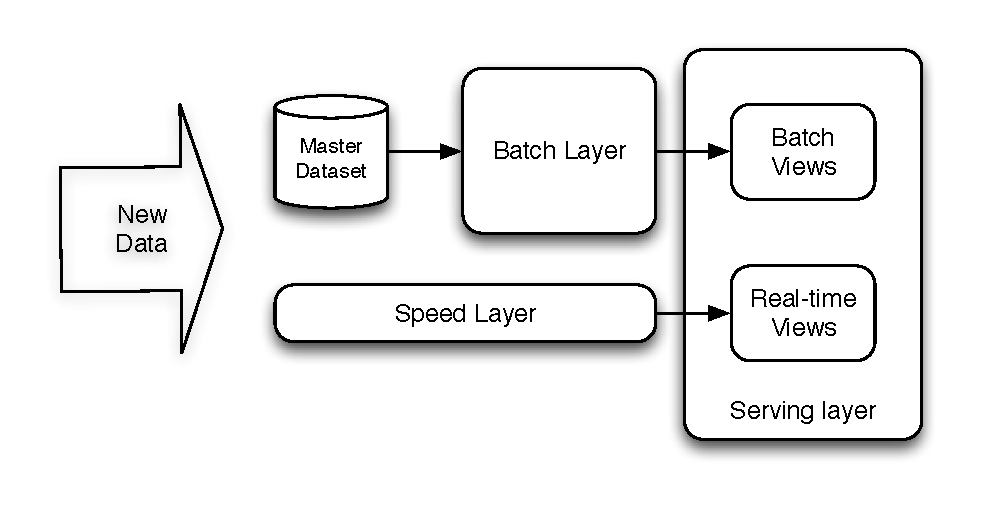
\epsfig{file=lambda.eps, height=2in, width=3in}
\caption{Lambda Architecture.}
\label{fig:lambda}
\end{figure}

In the following subsections we will examine how the different components
of the Lambda architecture can be implemented with Spring XD.

\subsubsection {Master dataset with Spring XD}

While Spring XD does not provide a storage mechanism of its own, it
integrates with a variety of storage technologies, both for reading,
via source modules (see~\ref{sec:Source}), as well as for writing, via
sink modules (see~\ref{sec:Sink}). A \emph{data ingestion}
stream can be used to consolidate data from external sources into
central storage.

For example, the following stream definition can be used to ingest 
MQTT\cite{mqtt} data sent by a number of sensors directly into HDFS:

\verb;stream create ingest --definition "mqtt | hdfs";

In a more elaborate setting, an application can collect data from
different sources, and Spring XD can provide the means to merge them
in a single master dataset. The streams \texttt{in-mqtt} and \texttt{in-http}
collect data from sensors via MQTT and HTTP, respectively, and
contribute to a single queue \texttt{hdfs-in}. The merged result
is saved into HDFS.

\verb;stream create in-mqtt --definition ;\\*
\verb;  "mqtt > queue:hdfs-in";

\verb;stream create in-http --definition  ;\\*
\verb;  "http > queue:hdfs-in";

\verb;stream create ingest --definition  ;\\*
\verb;  "queue:hdfs-in > hdfs";

\subsubsection {Batch layer in Spring XD}

Once data is collected into the \emph{master dataset}, it can be processed
by \emph{jobs} (see~\ref{sec:Job}). The similarities between Spring XD's
notion of a \emph{job} and Lambda Architecture's corresponding notion of
a \emph{batch job} make the mapping straightforward.


The data ingested in the master dataset can be consumed by a batch job,
created as follows:

\verb;job create sensorProcess;\\*
\verb;  --definition "sensors";

(This example already assumes an existing module job named \emph{sensors} that
implements the processing logic).

Spring XD supports the partitioning of jobs for concurrent execution on
separate containers. This allows for increased throughput and reduced latency
for job executions. Such execution parameters are defined during deployment,
as follows:

\verb;job deploy sensor-process;\\*
\verb;  --properties module.sensorProcess.count=3;

An important characteristic of the \emph{batch layer} is the regular
execution of jobs, as well as the ability to replay older datasets, for
instance reconstructing the \emph{data views} in case of loss or error.
For that, Spring XD provides the following mechanisms:

\begin{itemize*}
\item \emph{manual} job launch through its shell user interface or 
administrative UI;
\item \emph{stream-controlled} where the jobs are launched by a stream of 
\emph{trigger} messages;
\item \emph{scheduled} job launch according to a \texttt{cron} expression;
\end{itemize*}

For example, a job can be launched manually as follows:

\verb;job launch sensor-process;

Or, more typically, it can be launched on a schedule:

\verb;stream create --name launchSensorProcess;\\*
\verb;  --definition "trigger --cron=`0/5 * * * * *';\\* 
\verb;  > queue:job:myCronJob" --deploy;

\subsubsection {Speed layer in Spring XD}

The role of the \emph{speed layer} is to complement the \emph{batch layer} 
by performing real-time computations on the incoming data, thus filling the 
inherent latency gap. This functionality can be implemented in Spring XD by 
its analytics support (see section~\ref{sec:Analytics}).

Considering the previous example, while ingesting data from sensors and 
populating the master dataset, the application may perform various computations 
on the data stream. For example, it can perform a count of the incoming elements. 

\verb;stream create count --definition  ;\\*
\verb;"tap:stream:ingest > aggregate-counter";

In a more elaborate scenario, it is possible to actually do 
some processing of the data in-flight and store the results in real-time views
for being combined with the batch views.

\verb;stream create count --definition  ;\\*
\verb;"tap:stream:ingest > extract-tags | jdbc";

\subsubsection {Serving layer with Spring XD}

Spring XD provides out-of-the box RESTful services for its counters and gauges,
which can operate as part of the serving layer. In addition to that,  
the data stored by the \emph{batch jobs} in the 
\emph{batch views}, as well as \emph{real time views} produced by the streams, 
can be easily made available through a serving layer using Spring Boot \cite{spring-boot},
in combination with Spring Data \cite{spring-data} or Spring Data REST \cite{spring-data-rest}.

\subsection {Reactive applications}

The last few years have seen a significant change in application requirements:
data volumes of terabyte order, response times within tens of milliseconds, stricter
availability requirements. These new challenges require a new approach to application
development, subsumed under the concepts of \emph{reactive applications} and \emph{reactive
programming}. In what follows next, we will describe how these concepts are
illustrated by Spring XD, both from a runtime platform, as well as from a development perspective.

\subsubsection {Spring XD as a platform for \\ reactive applications}

Reactive applications, as described by the Reactive \linebreak Manifesto
\cite{reactive} are \emph{responsive}, \emph{resilient}, \emph{elastic}
and \emph{message driven}. Spring XD, as a platform, provides the means for creating and
running reactive applications.

\emph{Responsiveness} represents a system's ability to respond in a timely manner, if
at all, possible. In the case of Spring XD, its stream processing model is designed
for building fast, low-latency data pipelines.

\emph{Resilience} represents a system's ability to remain responsive in the face of
failure. In Spring XD, this is provided out of the box by features such as automatic
module redeployment if the host container has crashed, or the ability to elect a new
admin node in case the existing one fails. On a more granular level, automatic retry
and dead-letter queue support for RabbitMQ and Redis allows tracking and recovery
from failed computations. The use of messaging middleware ensures redelivery of data
when a module recovers.

\emph{Elasticity} represents a system's ability to remain responsive under varying
workload. In Spring XD, this is provided by features such as the ability to scale up
the processing power by deploying multiple instances of a module or job in a stream.
The use of messaging middleware provides backpressure allowing each component in the
stream to consume data at its own pace.

\emph{Message-driven} represents a system's reliance on \linebreak
asynchronous message passing between components. This is a core
feature of Spring XD, implemented by its message bus (see~\ref{subsec:MessageBus}).

This is how Spring XD as a platform allows applications to meet the criteria for being
considered \emph{reactive}. In conjunction with that, it provides the ability of using
a development model that is better suited for reactive applications, through its support
for \emph{reactive programming} and \emph{observable streams}.

\subsubsection {Reactive programming and functional \\ in Spring XD}

\emph{Reactive programming} is a programming paradigm centered around asynchronous
stream processing. The central notion is that incoming data can be processed in an
ordered, asynchronous and event-driven manner, using functional operators to describe
transformations that apply to an entire stream of incoming data. The operators can
vary from individual item transformations, to grouping and aggregation over given
time windows, and can be composed into complex data processing pipelines that produce
outbound streams of data.

ReactiveX~\cite{reactivex} is one of the most common set of APIs, centered around
the \texttt{Observable} abstraction that extends the observer pattern to streams,
together with a rich set of operators for composing and transforming sequences, and
RxJava~\cite{rxjava} is the Java implementation of the ReactiveX API. Another
reactive programming library for Java is provided by Project 
Reactor~\cite{reactor}, whose abstraction is called a \texttt{Stream}.
Reactive Streams~\cite{reactivestreams} is an initiative to provide a standard for
asynchronous stream processing with non-blocking backpressure (the ability of the
consumers to regulate the data flow and instruct the producers to adjust their
production rate) on the JVM.

Spring XD provides support for reactive programming \linebreak
through a special type of processors that transform asynchronous
streams of data. Both the APIs for RxJava and Project Reactor are
supported. An example of an RxJava processor is shown in
figure \ref{fig:rxjava}, and Reactor integration is almost identical. Spring XD
has the responsibility of transforming the flow of discrete messages arriving
on a processor's input channel into an RxJava \texttt{Observable}, as well as
transforming the \texttt{Observable} returned by the processor module into a
flow of discrete messages sent on the output channel. Inside the processor,
RxJava operators are applied for performing transformations on the data stream.

\begin{figure}[ht]
\centering
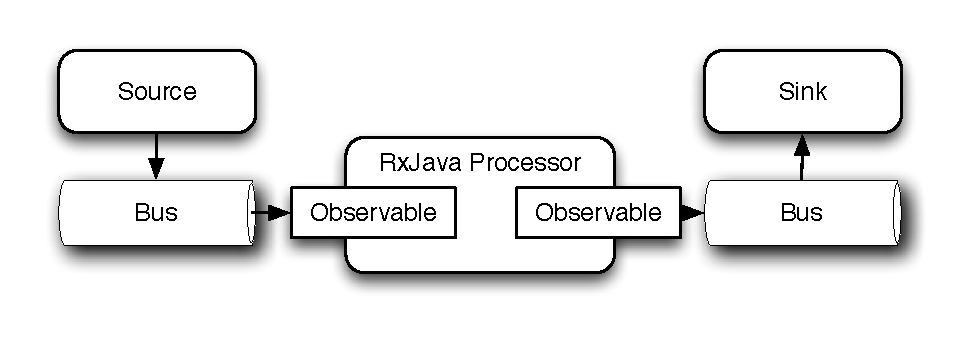
\epsfig{file=rxjava.eps, height=2in, width=3in}
\caption{Reactive module using RxJava}
\label{fig:rxjava}
\end{figure}

